\documentclass[a4paper,12pt]{article}
%%%%%%%%%%%%%%%%%%%%%%%%%%%%%%%%%%%%%%%%%%%%%%%%%%%%%%%%%%%%%%%%%%%%%%%%%%%%%%%%%%%%%%%%%%%%%%%%%%%%%%%%%%%%%%%%%%%%%%%%%%%%%%%%%%%%%%%%%%%%%%%%%%%%%%%%%%%%%%%%%%%%%%%%%%%%%%%%%%%%%%%%%%%%%%%%%%%%%%%%%%%%%%%%%%%%%%%%%%%%%%%%%%%%%%%%%%%%%%%%%%%%%%%%%%%%
\usepackage{eurosym}
\usepackage{vmargin}
\usepackage{amsmath}
\usepackage{graphics}
\usepackage{epsfig}
\usepackage{enumerate}
\usepackage{multicol}
\usepackage{subfigure}
\usepackage{fancyhdr}
\usepackage{listings}
\usepackage{framed}
\usepackage{graphicx}
\usepackage{amsmath}
\usepackage{chngpage}
%\usepackage{bigints}

\usepackage{vmargin}
% left top textwidth textheight headheight
% headsep footheight footskip
\setmargins{2.0cm}{2.5cm}{16 cm}{22cm}{0.5cm}{0cm}{1cm}{1cm}
\renewcommand{\baselinestretch}{1.3}

\setcounter{MaxMatrixCols}{10}
\begin{document}
\begin{enumerate}



\item Suppose that the results of an experimental procedure resulted in the collection of datasets $X$ and $Y$. Consider the following inference procedure performed on data set $X$.
\begin{center}
\begin{framed}
	\begin{verbatim}
	> shapiro.test(X)
	
	Shapiro-Wilk normality test
	
	data:  X
	W = 0.9619, p-value = 0.6671
	
	\end{verbatim}
\end{framed}
\end{center}


\begin{itemize}
	\item[(a)]  Describe the purpose of this procedure.
	\item[(b)]  What is the null and alternative hypothesis?
	\item[(c)]  What is your conclusion about this procedure?
\end{itemize}


% - Question 4

% Inference for Single Samples

\item

\begin{enumerate}[(a)]

\item Answer the following theory questions on hypothesis testing.
\begin{enumerate}[(i)]
\item  In the context of hypothesis testing, explain what a p-value is, and how it is used. Support your answer with a simple example.
\item  What is meant by Type I error and Type II error?
\end{enumerate}

 %====================================================%
 
\item Suppose that the results of an experimental procedure resulted in the collection of datasets $X$ and $Y$. Consider the following inference procedure performed on data set $X$.
\begin{center}
\begin{framed}
\begin{verbatim}
> shapiro.test(X)

        Shapiro-Wilk normality test

data:  X
W = 0.77516, p-value = 0.0003767
\end{verbatim}
\end{framed}
\end{center}


\begin{itemize}
	\item[(i)]  Describe the purpose of this procedure.
	\item[(ii)]  What is the null and alternative hypothesis?
	\item[(iii)]  What is your conclusion about this procedure?
\end{itemize}
\smallskip

 A graphical procedure was carried out to assess whether or not this assumption of normality is valid for data set \texttt{Y}. Consider the Q-Q plot in the figure below.

\begin{center}
	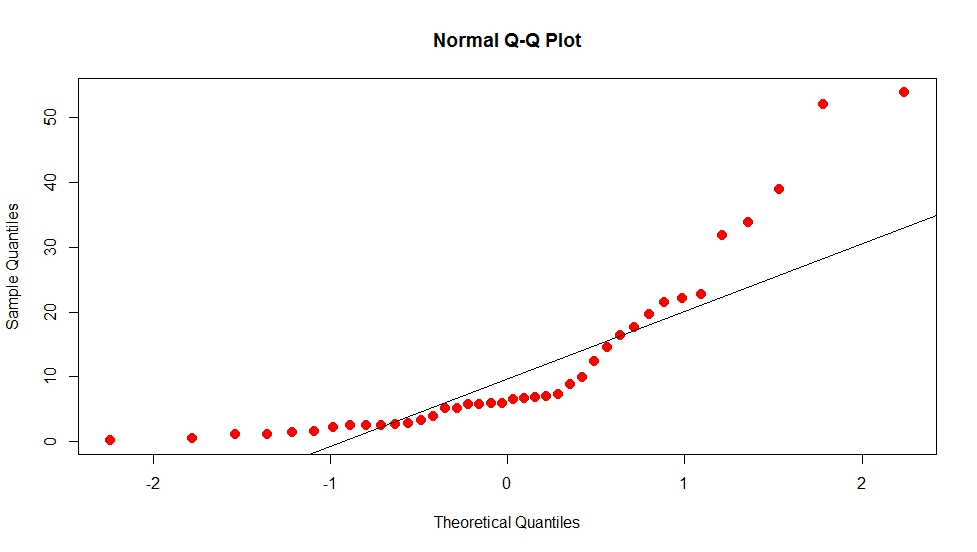
\includegraphics[scale=0.40]{images/qqplot2}
\end{center}

\begin{itemize}
	\item[(iv)]  Provide a brief description on how to interpret this plot.
	\item[(iv)]  What is your conclusion for this procedure? Justify your answer.
\end{itemize}
\end{enumerate}
\newpage


% Part A - Dixon Q Test (5 Marks)
\item Use the Dixon Q-test to determine if there is an outlier present in this sample data. You may assume
a significance level of 5\%.
\[ 131, 139, 155, 127, 123, 
  134, 140, 122, 132, 135\]
\begin{enumerate}[(i)]
\item  State the null and alternative hypotheses for this test.
\item Compute the test statistic?
\item  State the appropriate critical value.
\item  What is your conclusion to this procedure?
\end{enumerate}

\end{enumerate}

\end{document}
